
\chapter{Chapter Heading}

\abstract*{As cybersecurity defenses strengthen, attackers increasingly turn to social engineering to exploit, or hack the human element of security systems. By manipulating trust, psychology, and behavior, cybercriminals bypass technical safeguards to gain unauthorized access to networks. Social engineering is particularly effective because it is often easier to compromise a person than it is to discover a system vulnerability, for example. These attacks are becoming incresingly difficult to counter since they lack consistent patterns and can be tailored to specific individuals or organizations. As a result, social engineering has become one of the most pervasive and dangerous forms of cyberattack. This chapter analyzes the methods and tactics used in recent social engineering incidents, highlights common human  behaviroal elements and vulnerabilities that can be exploited by attackers, and reviews current defense strategies. Emerging approaches-such as \textit{Machine Learning (ML)}detection methods-are also examined as potential solutions for reducing the effectiveness of these attacks.}

\abstract{As cybersecurity defenses strengthen, attackers increasingly turn to social engineering to exploit, or hack the human element of security systems. By manipulating trust, psychology, and behavior, cybercriminals bypass technical safeguards to gain unauthorized access to networks. Social engineering is particularly effective because it is often easier to compromise a person than it is to discover a system vulnerability, for example. These attacks are becoming incresingly difficult to counter since they lack consistent patterns and can be tailored to specific individuals or organizations. As a result, social engineering has become one of the most pervasive and dangerous forms of cyberattack. This chapter analyzes the methods and tactics used in recent social engineering incidents, highlights common human  behaviroal elements and vulnerabilities that can be exploited by attackers, and reviews current defense strategies. Emerging approaches-such as \textit{Machine Learning (ML)}detection methods-are also examined as potential solutions for reducing the effectiveness of these attacks.}

\section{Introduction}
The digital world is expanding as we know it, and is doing so at an alarming pace, with the internet now central to communications, business transactions, knowledge sharing, and entertainment; however, this rapid growth has also raised serious concerns about user security and privacy and despite increasingly sophisticated defenses being employed, many cyberattacks still succeed by exploiting these flaws, such as application design flaws, technical weaknesses, or deception-based methods. Among these, \textit{scamming and phishing}-forms of social engineering (SE) attacks-remain especially prevalent.

Social engineering attacks exploit, or hack human vulnerabilities playing off of human weaknesses such as deception, persuasion, manipulation, and influence. These weaknesses are then leveraged for nefarious purposes and reasons all dependant upon the attacker's goals, objectives, and mission. Most of these attacks aim to harvest information containing confidential information, unauthorized access, or insights into an organization's internal and external perimeter defeneses. A key challenge in mitigating SE-based attacks is their lack of consistent patterns; in many cases, even the victim may not realize they are being manipulated. As a result, traditional countermeasures often struggle to detect or prevent such attacks.

In recent years, several high-profile breaches have demonstrated how attackers exploit the human element in cybersecurity. Despite advances in technical safeguards, people remain a critical and vulnerable link in the security chain. Figure 1 illustrates common tools and the general flow of social engineering-based cyberattacks.

\begin{figure}
    \centering
    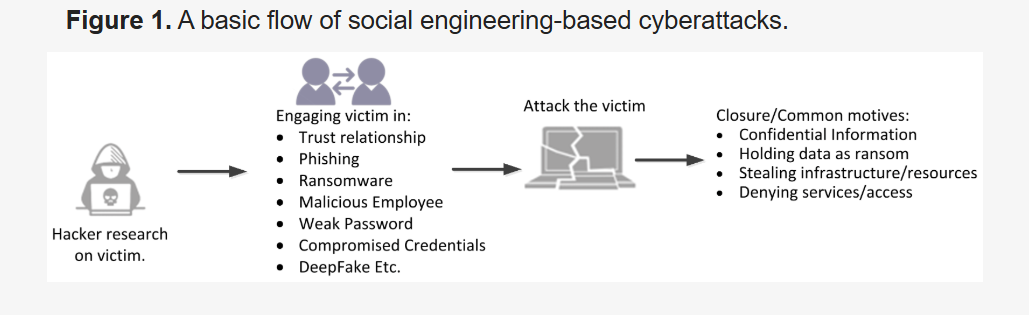
\includegraphics[width=1\linewidth]{soceng.png}
    \caption{Enter Caption}
    \label{fig:placeholder}
\end{figure}
In the past two years, the most common mediums for conducting social engineering (SE) attacks have been through the use of social media platforms and \textit{smishing}(SMS-based phishing) campaigns. The majority of SE attacks depend on direct interactions between the attacker and the victim. In many cases, these interactions can be deceptively simple-for example, a phone call in which an attacker impersonates an employee to extract sensitive information such as passwords or PIN codes. The scale of this threat is evident in recent statistics: in 2024 alone, Americans lost an estimated USD 29.8 billion to phone scame alone.

Table 1 provides an overview of several prominent social engineering-based breaches from recent years. These incidents highlight the dual role of \textit{human error} and \textit{delivberate attacker manipulation} in enabling successful compromise. SE attacks often succeed by persuading or coercing a victim into making an error they would not otherwise commit, demonstrating that technical defenses alone are insufficient.

Beyond direct financial loss, data breaches resulting from SE attacks erode customer trust, loyalty, and damage organizational brand and reputation. Despite the high impact and relative ease of execution, countermeasures for SE-based attacks often overlook the critical link between \textit{human behavior} and \textit{social manipulation techniques.} Few studies directly address this intersection. This chapter seeks to extend that body of knowledge by analyzing human behaviroal vulnerabilities and how they are exploited in SE-based attacks.

The remaining parts of this chapter is structured as follows: Section 2 reviews well-known social engineering indicents and their methods of execution. Section 3 discusses common human emotions and errors exploited in SE attacks, along with current countermeasures and the role of Machine Learning (ML). Section 4 highlights the limitations of existing approaches and summarizes the finding of this study. Finally, Section  5 concludes this chapter.

\begin{table}
    \centering
    \begin{tabular}{cccc}
         Company&  Date&  Details / Damage& Breach Method / Tool\\
         MGM Resorts Las Vegas International&  September 2023&  Attackers used vishing (phone call) to trick help desk personnel into resetting an account. Led to ransomware deployment, disrupting hotel operations, slot machines, and reservations. Estimated damages exceeded US 100 million& Vishing (help desk impersonation), phishing, ransomware (ALPHV / BlackCat)\\
         Caesars Entertainment, Las Vegas, NV&  September 2023&  Similar social engineering campaign as MGM; attackers stole data including driver's license and SSNs of loyalty program members. Caesars reportedly paid the US 15 million ransom& Phishing + social engineering of hotel IT staff\\
         Okta (Identity Provider)&  October 2023&  Attackers gained access to Okta's customer support case system by tricking employees. Breach impacted customers like Cloudflare and BeyondTrust& Phishing + Credential Theft\\
       Coinbase& February 2023& Employees targeted with SMS phishing (Smishing) that led to credential harvesting. Attackers stole login details and gained limited system access. Customer funds were not stolen& Smishing + Credential Phishing\\
       Reddit& February 2023& Employee fell for a targeted phishing email mimicking internal HR portal. Attackers stole credentials and internal documentation& Spearphishing Email \\
       Microsoft (Storm-0558)& Mid-2023& Chinese threat actors spear-phished and stole a signing key, allowing them to forge tokens to access U.S. government email accounts (including State Dept.)& Spearphishing + Forgery\\
       Western Digital& April 2023& Attackers gained access to internal systems via social engineering. Customer data and cloud services disrupted& Phishing / SE + Ransomware\\
       Lufthansa Group (Airline)& 2024 (reported)& Smishing campaigns targeted frequent flier program members, tricking them into revealing credentials. Accounts hijacked for resale& Smishing\\
       Ticketmaster (via Snowflake Compromise)& 2024& Attackers used stolen credentials from social engineering / credential stuffing against Snowflake accounts, exfiltrating 560M customer records& Credential Phishing + Credential Reuse\\
       UnitedHealth Group (Change Healthcare)& February 2024& Attackers from ALPHV / BlackCat gained access via stolen credentials, likely from phishing, leading to massive ransomware attacks disrupting healthcare services nationwide& Phishing + Credential Theft\\
       AT&T Data Breach& 2024& SIM-swapping and phishing techniques used to compromise employee access. Millions of customer records were exposed& Phishing + SIM-Swapping\\
       Cisco Talos& 2025 (ongoing)& Multiple campaigns using MFA fatigue and phishing to target corporate VPN users across industries& MFA Fatigue attack + Phishing
    \end{tabular}
    \caption{Caption}
    \label{tab:placeholder}
\end{table}

\section{Social Engineering Attacks}
Social engineering (SE) can be defined as the exploitation of human psychology to achieve malicious objectives, rather than relying on purely technical hacking methods. As society's dependence on technology grows, SE has become an increasingly important tool for cybercriminals. At the same time, technical countermeasures against cyberattacks-such as intrusion detection systems, firewalls, and endpoint protection-have advanced significantly. These defenses make purely technical intrusions more difficult to execute, thereby pushing attackers toward exploiting the human element as a more reliable entry point.

SE-based attacks can assist adversaries in multiple ways, including infiltrating organizational networks, bypassing firewalls, installing malware, or creating backdoors for persistent access. Unlike technical vulnerabilities, SE attacks target human decision-making processes and behaviors. For example, attackers may induce victims to make errors by exploiting cognitive biases or pressuring them into hasty actions. Similarly, traits such as curiosity, fear, or trust can be manipulated to extract sensitive information and foretelling details. This section examines several of the most common cyberattacks enabled by social engineering.

\subsection{Phishing Attacks}
Phishing is one of the most prevalent and successful forms of SE-based cyberattacks. Every day, millions of fraudulent emails are distributed by attackers or spam bots, with many intercepted by security solutions but a significant portion still reaching users. A phishing campaign typically begins with an email crafted to appear as though it originates from a legitimate party or source. The goal is to lure the victim into taking and completing an action that compromises the security of not only themselves, but for others as well.

The lure varies depending on the target audience: a corporate employee may receive a fake travel expense report requiring a login, while another user may be promised a prize for clicking a malicious link. Regardless of the delivery method, the ultimate aim of phishing is to steal sensitive information, such as login credentials, financial details, or \textit{Personally Identifiable Information (PII).}

Figure 2 illustrates the general process of a basic phishing attack, including two of the most common methods. Table 2 further categorizes different phishing techniques and highlights their key characteristics.

\begin{figure}
    \centering
    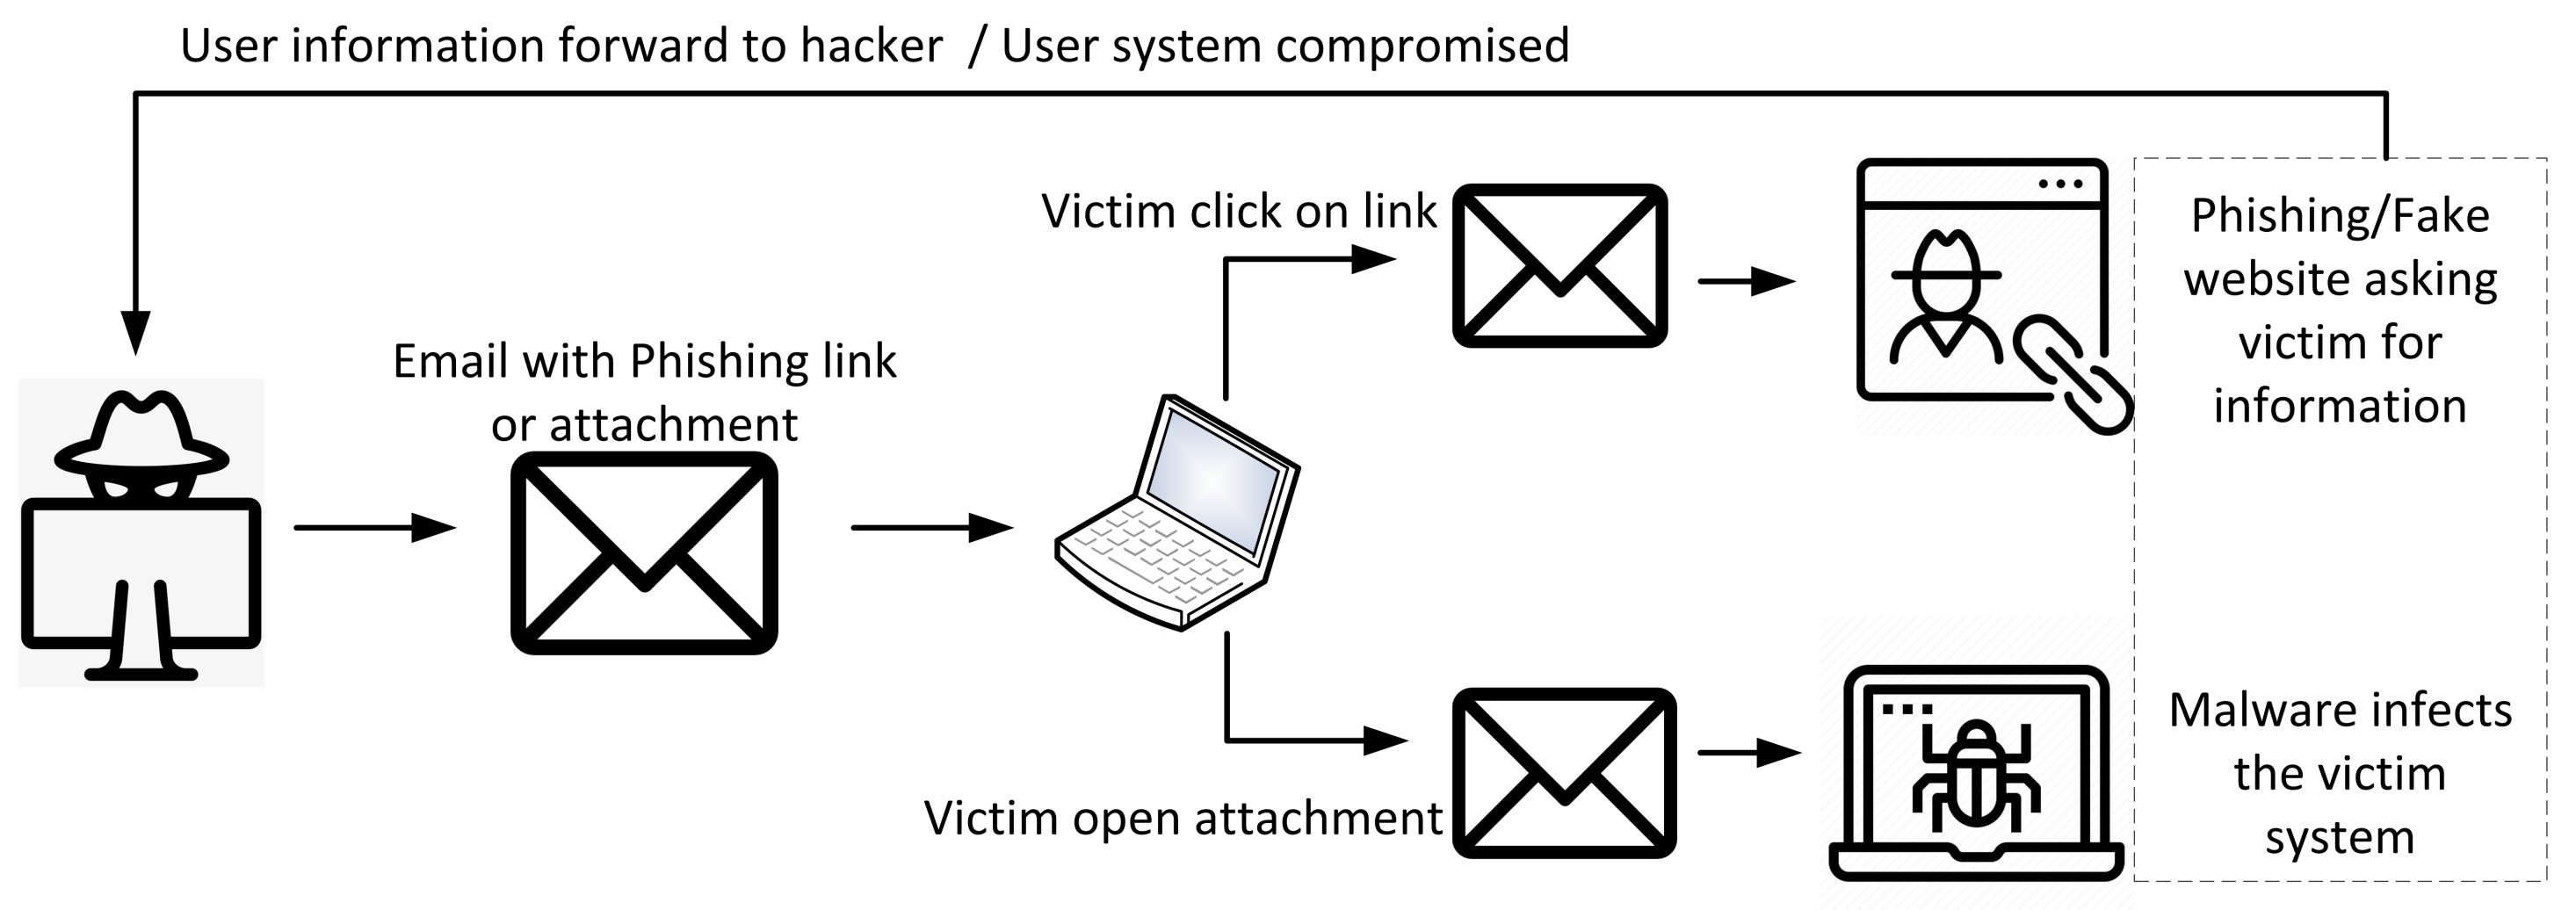
\includegraphics[width=1\linewidth]{phish.png}
    \caption{\textbf{FIGURE 2. }Common phishing attack workflow}
    \label{fig:placeholder}
\end{figure}
\subsubsection{Table 2. Common Types of Phishing Attacks}


\begin{table}
    \centering
    \begin{tabular}{cc}
         Phishing Attack& Description\\
         Spear& A spearphishing attack is a highly targeted, personalized scam designed to trick specific individuals or organizations into revealing sensitive information. Unlike a generic phishing attempt that casts a wide net, Spearphishers meticulously research their targets to craft convincing emails hat appear to come from a trusted source, such as a colleague, vendor, or executive.\\
         Whaling& A whaling attack is a highly targeted form of phishing that specifically goes after high-level executives and key decision-makers within an organization. Like hunting a "big fish," attackers focus on these "whales" because of their authority and access to valuable data and significant funds. The goal is to manipulate them into revealing sensitive information or transferring large sums of money to fraudulent accounts.\\
         Vishing& Vishing is a type of cybercrime in which attackers use deceptive phone calls and voicemail messages to manipulate individuals into disclosing sensitive personal information, such as bank account details, credit card numbers, Social Security numbers, or login credentials. It is essentially the "voice" version of phishing, where scammers typically impersonate representatives from trusted organizations, such as banks, government agencies (such as the IRS or Social Security Administration), tech support, or even family members.\\
         Smishing& Smishing is a form of cybercrime that uses deceptive text messages to trick individuals into giving up sensitive information, downloading malware, or sending money. The name is a blend of "SMS" (Short Message Service) and "phishing." Smishing attacks are effective because people tend to be less skeptical of text messages compared to emails and often respond to them with a great sense of urgency.\\
         Impersonation& An impersonation attack is a form of social engineering in which a cybercriminal pretends to be a known or trusted person or entity to deceive a victim. The attacker's goal is to manipulate the target into taking actions that benefit the criminal, such as transferring funds, sharing sensitive information, or revealing login credentials. Unlike malware-based attacks that exploit software vulnerabilities, impersonation attacks exploit human psychology and a person's natural tendency to trust. They can occur through various methods and means, both digital and physical.\\
         Business Email Compromise (BEC)& Business Email Compromise (BEC) is a sophisticated type of cybercrime where attackers use email to impersonate a trusted individual or organization, such as a CEO, vendor, or legal counsel, to trick employees into taking actions that benefit the attacker, such as wiring funds or sharing sensitive information.\\
         Clone Phishing& Clone phishing is a cyberattack where an attacker creates a nearly identical copy of a legitimate, previously-sent email to deceive recipients. By perfectly replicating the branding, language, and sender details, the attacker replaces original links or attachments with malicious ones. This tactic exploits a victim's trust in a familiar source, making the fraudulent email very difficult to detect.\\
         Social Media Phishing& Social media phishing is a cyberattack that uses social networking platforms to trick users into revealing sensitive information, such as passwords, credit card numbers, and other personal data. Threat actors create fake profiles, send malicious links, or hack legitimate accounts to deceive victims and exploit their trust in familiar platforms.\\
         Distributed Spam Distraction (DSD)& Distributed Spam Distraction (DSD) is a cyberattack in which a user's inbox is flooded with thousands of non-malicious emails to distract them from more serious criminal activities happening in the background. This deluge of spam, often from thousands of different senders, serves as a smokescreen to hide alerts about fraudulent purchases or account changes. The attack relies on the fact that a user's attention is limited. By overwhelming the inbox with junk email, attackers hope the victim will miss the few critical, legitimate-seeming emails from banks or other financial institutions reporting unauthorized activity.\\
    \end{tabular}
    \caption{Caption}
    \label{tab:placeholder}
\end{table}
\subsection{Dumpster Diving}
Dumpster diving is a low-tech yet effective method used to gather information about a target by searching through discarded materials such as trash or recycling bins. Attackers look for documents, receipts, notes, or other items that may contain sensitive data-including passwords, payslips, bills, credit card details, PII, or internal organizational information such as intellectual property and proprietary information, or trade secrets.

Even seemingly insignificant scraps of paper can reveal critical data that may aid in planning or executing social engineering (SE) attacks. This method is also one of the most common tactics used in identity theft.

Figure 3 illustrates the types of materials commonly found in organization's dumpster. These items are often carelessly disposed of without proper shredding, sanitization, or secure disposal, allowing malicious actors to retrieve and exploit the information for SE-based attacks.

\begin{figure}
    \centering
    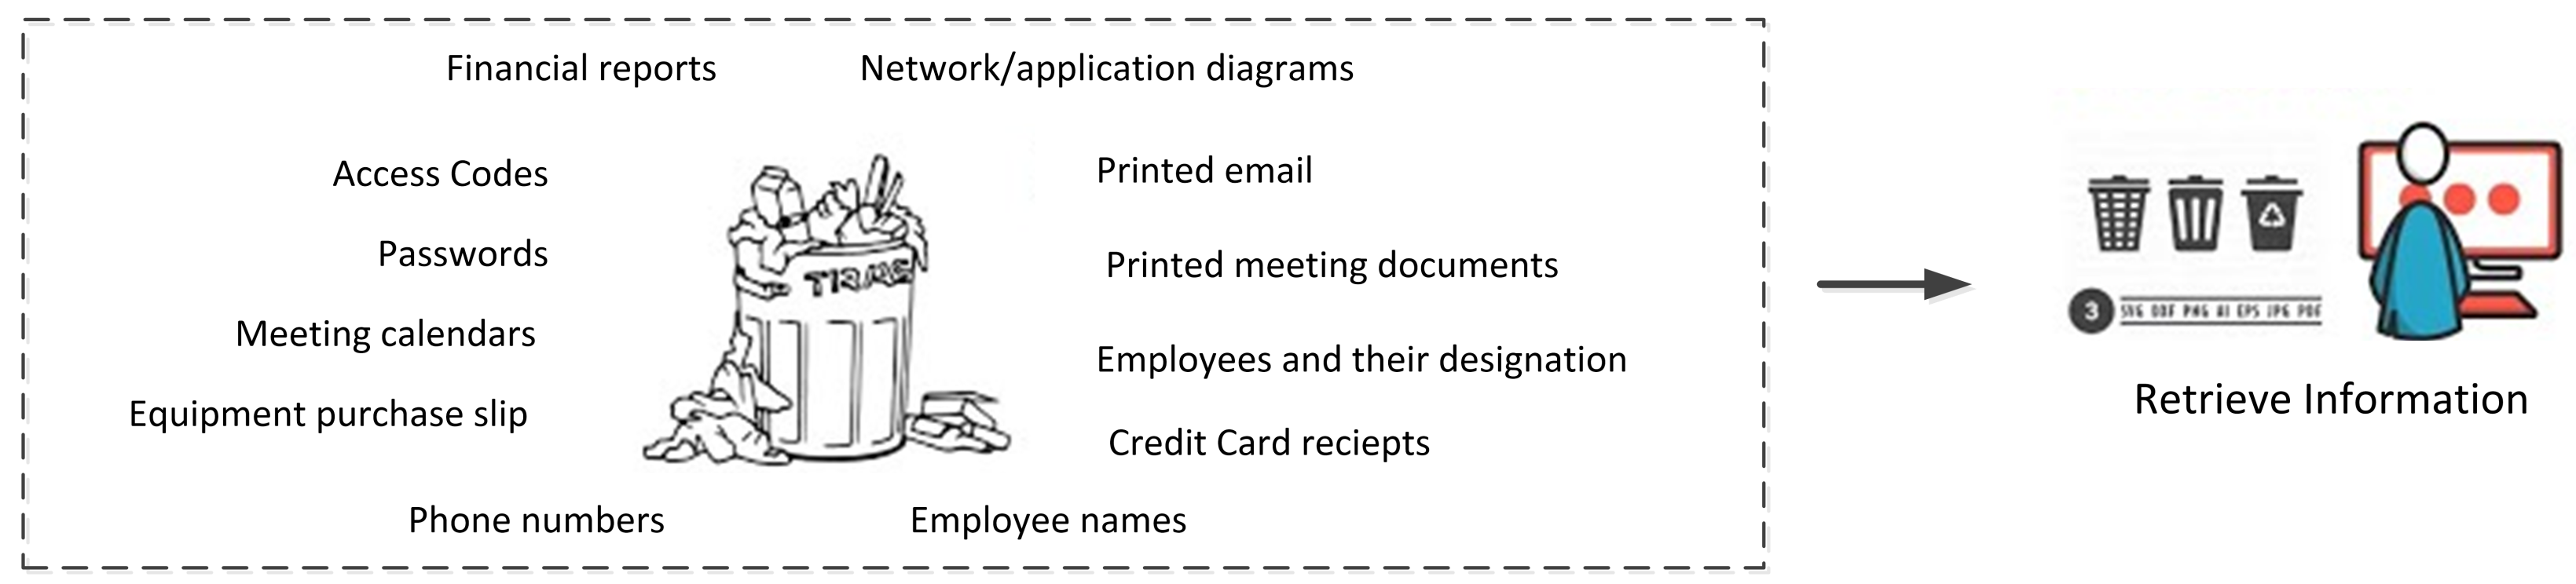
\includegraphics[width=0.75\linewidth]{dumpsterdive.png}
    \caption{Enter Caption}
    \label{fig:placeholder}
\end{figure}

















\section{Section Heading}
Instead of simply listing headings of different levels we recommend to let every heading be followed by at least a short passage of text. Furtheron please use the \LaTeX\ automatism for all your cross-references and citations.


\subsection{Subsection Heading}

Instead of simply listing headings of different levels we recommend to let every heading be followed by at least a short passage of text. Further on please use the \LaTeX\ automatism for all your cross-references\index{cross-references} and citations\index{citations} as has already been described in Sect.~
\subsubsection{Subsubsection Heading}
Instead of simply listing headings of different levels we recommend to let every heading be followed by at least a short passage of text. Furtheron please use the \LaTeX\ automatism for all your cross-references and citations as has already been described in Sect., see also Fig.~\ref{fig:1}\footnote{If you copy text passages, figures, or tables from other works, you must obtain \textit{permission} from the copyright holder (usually the original publisher). Please enclose the signed permission with the manucript. The sources\index{permission to print} must be acknowledged either in the captions, as footnotes or in a separate section of the book.}

Please note that the first line of text that follows a heading is not indented, whereas the first lines of all subsequent paragraphs are.

references and citations citations as has already been described in Sect.

Please note that the first line of text that follows a heading is not indented, whereas the first lines of all subsequent paragraphs are.

\begin{svgraybox}
If you want to emphasize complete paragraphs of texts we recommend to use the newly defined Springer class option \verb|graybox| and the newly defined environment \verb|svgraybox|. This will produce a 15 percent screened box 'behind' your text.

If you want to emphasize complete paragraphs of texts we recommend to use the newly defined Springer class option and environment \verb|svgraybox|. This will produce a 15 percent screened box 'behind' your text.
\end{svgraybox}


\subsubsection{Subsubsection Heading}
Instead of simply listing headings of different levels we recommend to let every heading be followed by at least a short passage of text. Furtheron please use the \LaTeX\ automatism for all your cross-references and citations as has already been described in Sect.~\ref{ }.

Please note that the first line of text that follows a heading is not indented, whereas the first lines of all subsequent paragraphs are.

\begin{theorem}
Theorem text goes here.
\end{theorem}
%
% or
%
\begin{definition}
Definition text goes here.
\end{definition}

\begin{proof}
%\smartqed
Proof text goes here.
%\qed
\end{proof}

\paragraph{Paragraph Heading} %
Instead of simply listing headings of different levels we recommend to let every heading be followed by at least a short passage of text. Furtheron please use the \LaTeX\ automatism for all your cross-references and citations as has already been described in Sect.~\ref{ }.

Note that the first line of text that follows a heading is not indented, whereas the first lines of all subsequent paragraphs are.
%
% For built-in environments use
%
\begin{theorem}
Theorem text goes here.
\end{theorem}
%
\begin{definition}
Definition text goes here.
\end{definition}
%
\begin{proof}
%\smartqed
Proof text goes here.
%\qed
\end{proof}
%
%
\begin{trailer}{Trailer Head}
If you want to emphasize complete paragraphs of texts in an \verb|Trailer Head| we recommend to
use  \begin{verbatim}\begin{trailer}{Trailer Head}
...
\end{trailer}\end{verbatim}
\end{trailer}
%
\begin{question}{Questions}
If you want to emphasize complete paragraphs of texts in an \verb|Questions| we recommend to
use  \begin{verbatim}\begin{question}{Questions}
...
\end{question}\end{verbatim}
\end{question}
%
%
\begin{important}{Important}
If you want to emphasize complete paragraphs of texts in an \verb|Important| we recommend to
use  \begin{verbatim}\begin{important}{Important}
...
\end{important}\end{verbatim}
\end{important}
%
\clearpage
\begin{warning}{Attention}
If you want to emphasize complete paragraphs of texts in an \verb|Attention| we recommend to
use  \begin{verbatim}\begin{warning}{Attention}
...
\end{warning}\end{verbatim}
\end{warning}

\begin{programcode}{Program Code}
If you want to emphasize complete paragraphs of texts in an \verb|Program Code| we recommend to
use

\verb|\begin{programcode}{Program Code}|

\verb|\begin{verbatim}...\end{verbatim}|

\verb|\end{programcode}|

\end{programcode}
%
\begin{tips}{Tips}
If you want to emphasize complete paragraphs of texts in an \verb|Tips| we recommend to
use  \begin{verbatim}\begin{tips}{Tips}
...
\end{tips}\end{verbatim}
\end{tips}
%
\ifdefined\chapter\else\errmessage{This file must be included from the main document, not compiled on its own}\fi
%%%%%%%%%%%%%%%%%%%%%%%% referenc.tex %%%%%%%%%%%%%%%%%%%%%%%%%%%%%%
% sample references
% %
% Use this file as a template for your own input.
%
%%%%%%%%%%%%%%%%%%%%%%%% Springer-Verlag %%%%%%%%%%%%%%%%%%%%%%%%%%
%
% BibTeX users please use
% \bibliographystyle{}
% \bibliography{}
%
\biblstarthook{In view of the parallel print and (chapter-wise) online publication of your book at \url{www.springerlink.com}, it has been decided that -- as a general rule -- references should be sorted chapter-wise and placed at the end of the individual chapters. However, upon agreement with your contact at Springer, you may list your references in a single separate chapter at the end of your book. Deactivate the class option \texttt{sectrefs} and the \texttt{thebibliography} environment will be put out as a chapter of its own.}
References may be \textit{cited} in the text either by number (preferred) or by author/year.\footnote{Make sure that all references from the list are cited in the text. Those not cited should be moved to a separate \textit{Further Reading} section or chapter.} If the citatiion in the text is numbered, the reference list should be arranged in ascending order. If the citation in the text is author/year, the reference list should be \textit{sorted} alphabetically and if there are several works by the same author, the following order should be used:\begin{enumerate}
\item all works by the author alone, ordered chronologically by year of publication
\item all works by the author with a coauthor, ordered alphabetically by coauthor
\item all works by the author with several coauthors, ordered chronologically by year of publication.
\end{enumerate}
The \textit{styling} of references\footnote{Always use the standard abbreviation of a journal's name according to the ISSN \textit{List of Title Word Abbreviations}, see \url{http://www.issn.org/en/node/344}} depends on the subject of your book:
\begin{thebibliography}{99}
%
%
% Use the following syntax and markup for your references if 
% the subject of your book is from the field 
% "Mathematics, Physics, Statistics, Computer Science"
%
% Contribution 
\bibitem{humlinphil-journal} Author, Title, Journal, Year (placeholder for humlinphil-journal)
\bibitem{science-contrib} Broy, M.: Software engineering --- from auxiliary to key technologies. In: Broy, M., Dener, E. (eds.) Software Pioneers, pp. 10-13. Springer, Heidelberg (2002)
%
% Online Document
\bibitem{science-online} Dod, J.: Effective substances. In: The Dictionary of Substances and Their Effects. Royal Society of Chemistry (1999) Available via DIALOG. \url{http://www.rsc.org/dose/title of subordinate document. Cited 15 Jan 1999}
\protect\url{http://www.rsc.org/dose/title of subordinate document. Cited 15 Jan 1999}
%
% Monograph
\bibitem{science-mono} Geddes, K.O., Czapor, S.R., Labahn, G.: Algorithms for Computer Algebra. Kluwer, Boston (1992) 
%
% Journal article
\bibitem{science-journal} Hamburger, C.: Quasimonotonicity, regularity and duality for nonlinear systems of partial differential equations. Ann. Mat. Pura. Appl. \textbf{169}, 321--354 (1995)
%
% Journal article by DOI
\bibitem{science-DOI} Slifka, M.K., Whitton, J.L.: Clinical implications of dysregulated cytokine production. J. Mol. Med. (2000) doi: 10.1007/s001090000086 
%
% Use the following (APS) syntax and markup for your references if 
% the subject of your book is from the field 
% "Mathematics, Physics, Statistics, Computer Science"
%
% Online Document
\bibitem{phys-online} J. Dod, in \textit{The Dictionary of Substances and Their Effects}, Royal Society of Chemistry. (Available via DIALOG, 1999), 
\url{http://www.rsc.org/dose/title of subordinate document. Cited 15 Jan 1999}
%
% Monograph
\bibitem{phys-mono} H. Ibach, H. L\"uth, \textit{Solid-State Physics}, 2nd edn. (Springer, New York, 1996), pp. 45-56 
%
% Journal article
\bibitem{phys-journal} S. Preuss, A. Demchuk Jr., M. Stuke, Appl. Phys. A \textbf{61}
%
% Journal article by DOI
\bibitem{phys-DOI2} M.K. Slifka, J.L. Whitton, J. Mol. Med., doi: 10.1007/s001090000086
%
% Contribution 
\bibitem{phys-contrib} S.E. Smith, in \textit{Neuromuscular Junction}, ed. by E. Zaimis. Handbook of Experimental Pharmacology, vol 42 (Springer, Heidelberg, 1976), p. 593
%

%
% Use the following syntax and markup for your references if 
% the subject of your book is from the field 
% "Psychology, Social Sciences"
%
%
% Monograph
\bibitem{psysoc-mono} Calfee, R.~C., \& Valencia, R.~R. (1991). \textit{APA guide to preparing manuscripts for journal publication.} Washington, DC: American Psychological Association.
%
% Online Document
\bibitem{psysoc-online} Dod, J. (1999). Effective substances. In: The dictionary of substances and their effects. Royal Society of Chemistry. Available via DIALOG.

% Journal article
\bibitem{psysoc-journal} Harris, M., Karper, E., Stacks, G., Hoffman, D., DeNiro, R., Cruz, P., et al. (2001). Writing labs and the Hollywood connection. \textit{J Film} Writing, 44(3), 213--245.

% Contribution 
\bibitem{psysoc-contrib} O'Neil, J.~M., \& Egan, J. (1992). Men's and women's gender role journeys: Metaphor for healing, transition, and transformation. In B.~R. Wainrig (Ed.), \textit{Gender issues across the life cycle} (pp. 107--123). New York: Springer.

% Journal article by DOI
\bibitem{psysoc-DOI}Kreger, M., Brindis, C.D., Manuel, D.M., Sassoubre, L. (2007). Lessons learned in systems change initiatives: benchmarks and indicators. \textit{American Journal of Community Psychology}, doi: 10.1007/s10464-007-9108-14.

% Use the following syntax and markup for your references if 
% the subject of your book is from the field 
% "Humanities, Linguistics, Philosophy"
%
%
% Journal article

%
% Contribution 
\bibitem{humlinphil-contrib} Cameron, Deborah. 1997. Theoretical debates in feminist linguistics: Questions of sex and gender. In \textit{Gender and discourse}, ed. Ruth Wodak, 99--119. London: Sage Publications.
%

\bibitem{humlinphil-mono} Cameron, Deborah. 1985. \textit{Feminism and linguistic theory.} New York: St. Martin's Press.
%

\bibitem{humlinphil-online} Dod, Jake. 1999. Effective substances. In: The dictionary of substances and their effects. Royal Society of Chemistry. Available via DIALOG.
http://www.rsc.org/dose/title of subordinate document. Cited 15 Jan 1999

% Journal article by DOI
\bibitem{humlinphil-DOI} Suleiman, Camelia, Daniel C. O'Connell, and Sabine Kowal. 2002. `If you and I, if we, in this later day, lose that sacred fire...': Perspective in political interviews. \textit{Journal of Psycholinguistic Research}. doi: 10.1023/A:1015592129296.
% Use the following syntax and markup for your references if 
% the subject of your book is from the field 
% "Computer Science, Economics, Engineering, Geosciences, Life Sciences"
%
%
% Contribution 
\bibitem{basic-contrib} Brown B, Aaron M (2001) The politics of nature. In: Smith J (ed) The rise of modern genomics, 3rd edn. Wiley, New York 
%
% Online Document
\bibitem{basic-online} Dod J (1999) Effective Substances. In: The dictionary of substances and their effects. Royal Society of Chemistry. Available via DIALOG. 
%
% Journal article by DOI
\bibitem{basic-DOI} Slifka MK, Whitton JL (2000) Clinical implications of dysregulated cytokine production. J Mol Med, doi: 10.1007/s001090000086

% Journal article
\bibitem{basic-journal} Smith J, Jones M Jr, Houghton L et al (1999) Future of health insurance. N Engl J Med 965:325--329
%
% Monograph
\bibitem{basic-mono} South J, Blass B (2001) The future of modern genomics. Blackwell, London 
%
\end{thebibliography}

